\chapter{Reference Implementations}
\label{ch:implementation}

Chapter~\ref{ch:design} specified Saturn's protocol---a service type, a TXT record schema, a discovery flow, and a security posture. This chapter describes how I realized that design in code. I built three implementations in sequence under a fixed project timeline, each answering a question the previous one left open: Can Saturn bring AI to an application that has never had it? Can it provision AI at the network infrastructure layer? Can it handle the full complexity of agentic tool calling? All three build on a shared foundation of two packages I wrote. Both packages build on existing dependencies: the Python \texttt{zeroconf} library for mDNS advertisement and Vercel's AI SDK \texttt{ProviderV3} interface with the \texttt{multicast-dns} npm library for TypeScript discovery. On top of these, I built two original packages. The \texttt{saturn-ai} Python package\footnote{\url{https://github.com/jperrello/Saturn/tree/main/saturn}} adds ephemeral credential generation, OpenAI-compatible HTTP endpoints, and proxying to any upstream backend. The \texttt{ai-sdk-provider-saturn} npm package\footnote{\url{https://github.com/jperrello/Saturn/tree/main/ai-sdk-provider-saturn}} adds discovery orchestration, circuit breaking, and failover. These two packages use different mDNS libraries in different languages yet interoperate on the same service type and TXT record schema, supporting argument~\argref{A2}.

\section{VLC Extension: AI in a Non-AI-Native Application}
\label{sec:vlc-implementation}

A protocol that works only inside developer tools would be a weak demonstration of \argref{C1}.
VLC media player --- one of the most widely installed desktop applications --- has never offered AI features.
I chose it precisely for that reason: if Saturn can bring AI into VLC without the user configuring anything, the protocol demonstrates value beyond AI-native contexts.

\subsection{Architecture and Technology Choices}

VLC's extension system accepts only Lua scripts, and its HTTP support is limited to GET requests via \texttt{vlc.stream()}. No POST, no mDNS, no JSON library. These constraints ruled out embedding Saturn discovery directly in the extension.

I built a two-layer architecture.
A Lua extension (\texttt{saturn\_roast.lua}\footnote{\url{https://github.com/jperrello/Saturn/blob/main/vlc_extension/saturn_roast.lua}}, v1.0.0) provides the in-player GUI: a service dropdown, a single ``Roast Me!'' button, and styled HTML output.
I chose the roast variant over the conversational Saturn Chat extension because it better demonstrates the thesis claim: the user clicks one button, receives comedic commentary about their media choices, and never encounters a chat interface or any indication that a language model is involved.
A Python/FastAPI bridge (\texttt{vlc\_discovery\_bridge.py}\footnote{\url{https://github.com/jperrello/Saturn/blob/main/vlc_extension/vlc_discovery_bridge.py}}) runs as a background process, performing mDNS discovery and exposing an OpenAI-compatible REST API on localhost.
The bridge uses macOS's \texttt{dns-sd} CLI for discovery rather than the \texttt{zeroconf} library: a non-technical VLC user should install Saturn by copying a single directory, and bundling \texttt{zeroconf} into a standalone PyInstaller executable would add native dependencies that complicate that goal.

Two trade-offs follow from VLC's constraints.
Because Lua cannot POST, the extension sends request payloads as URL-encoded JSON in GET query parameters, which imposes URL length limits (typically 2,048 characters) on messages.
The bridge also requires a background Python process, adding a launch delay and a second process the user does not see.
I wrote a hand-written recursive descent JSON parser for Lua since VLC provides no JSON library.

I expect this bridge pattern to generalize: any application that can issue HTTP requests to the standard \texttt{/v1/} endpoints can integrate Saturn through a local bridge, though each bridge inherits platform-specific discovery costs and requires a background process.

When a user activates the extension (View $\rightarrow$ Extensions $\rightarrow$ Saturn Roast):

\begin{enumerate}
\item The extension locates the bundled bridge executable and launches it in the background with a \texttt{-{}-port-file} argument.
\item The bridge auto-detects an available port, starts the HTTP server, and writes \texttt{host:port} to the port file.
\item The extension polls the port file, then health-checks the bridge with exponential backoff (seven retries over approximately seven seconds).
\item Once ready, the extension queries \texttt{/services} to populate the service dropdown. The bridge browses \texttt{\_saturn.\_tcp.local.} every ten seconds in a background thread.
\item The user clicks ``Roast Me!'' The extension extracts media context --- title, artist, playback position --- via \texttt{vlc.input.item():metas()}, composes a single request with a system prompt instructing the model to roast the user's media taste, and the bridge proxies the request to the selected Saturn service. The model returns a short comedic response (capped at 200 tokens) with no persistent conversation history.
\end{enumerate}

Figure~\ref{fig:vlc-roast} shows the resulting dialog: the service dropdown, the ``Roast Me!'' button, and styled HTML output displaying the model's comedic commentary about the currently playing media.

\begin{figure}[H]
\centering
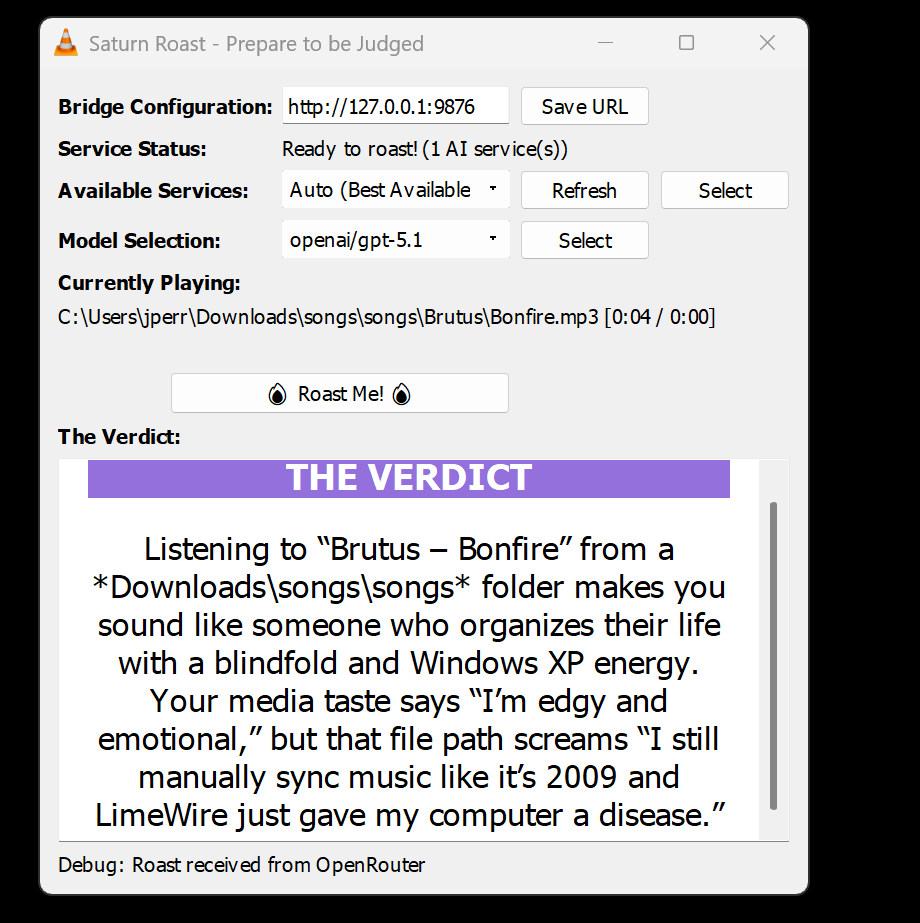
\includegraphics[width=0.75\textwidth]{figures/vlc-roast.png}
\caption{The Saturn Roast extension running inside VLC. The user selects a discovered service, clicks ``Roast Me!,'' and receives a short comedic roast of their media choices. No chat interface, model selector, or AI terminology is visible.}
\label{fig:vlc-roast}
\end{figure}

\section{Saturn Router: AI at the Network Infrastructure Layer}
\label{sec:router-implementation}

The VLC extension demonstrated that Saturn works in a consumer application.
The next question: could Saturn operate at the network level, embedded in the device that defines the network?
If Saturn runs on a router alongside DHCP and DNS, every device that joins the network gains AI access the same way it gains an IP address.

\subsection{Architecture and Technology Choices}

I structured the router implementation\footnote{\url{https://github.com/jperrello/Saturn/tree/main/saturn-router}} in three layers: a Rust binary managing the Saturn protocol, an OpenWRT integration layer embedding it into the router's service framework, and a LuCI web interface for browser-based administration.

The target hardware --- a GL.iNet GL-MT300N-V2 travel router with a MIPS32 processor and 128~MB of RAM --- cannot run a Python interpreter, so I made the choice to go with Rust. I scoped the build to this single router model; the binary cross-compiles to \texttt{mipsel-unknown-linux-musl} (a Rust Tier~3 target) using a Docker-based toolchain with soft-float musl and nightly \texttt{-Zbuild-std}.
Musl and MIPS32 constrained every dependency: \texttt{rustls} over \texttt{native-tls}, \texttt{attohttpc} over \texttt{reqwest} for a smaller binary, and aggressive size flags (\texttt{opt-level = "z"}, LTO, \texttt{panic = "abort"}).
Service registration uses the \texttt{mdns-sd} crate, a third independent mDNS library distinct from Python's \texttt{zeroconf} and JavaScript's \texttt{multicast-dns}.

The binary runs an event loop that ticks every 100 milliseconds: it health-checks upstream AI endpoints, rotates ephemeral credentials on schedule, and registers or unregisters the mDNS service based on backend availability.

I integrated the binary into OpenWRT using platform-native tooling: a \texttt{procd} init script manages process lifecycle with per-service JSON configuration files (permissions set to \texttt{600}), auto-downloading the binary from GitHub Releases if missing. A UCI schema exposes Saturn through the same \texttt{uci set}/\texttt{uci commit} workflow administrators use for firewall rules and DHCP. The LuCI web layer adds field validation, dynamic form visibility, and live status badges under the ``Services'' menu alongside DHCP and DNS.

Figure~\ref{fig:luci-config} shows the LuCI configuration page with its status badges.

\begin{figure}[H]
\centering
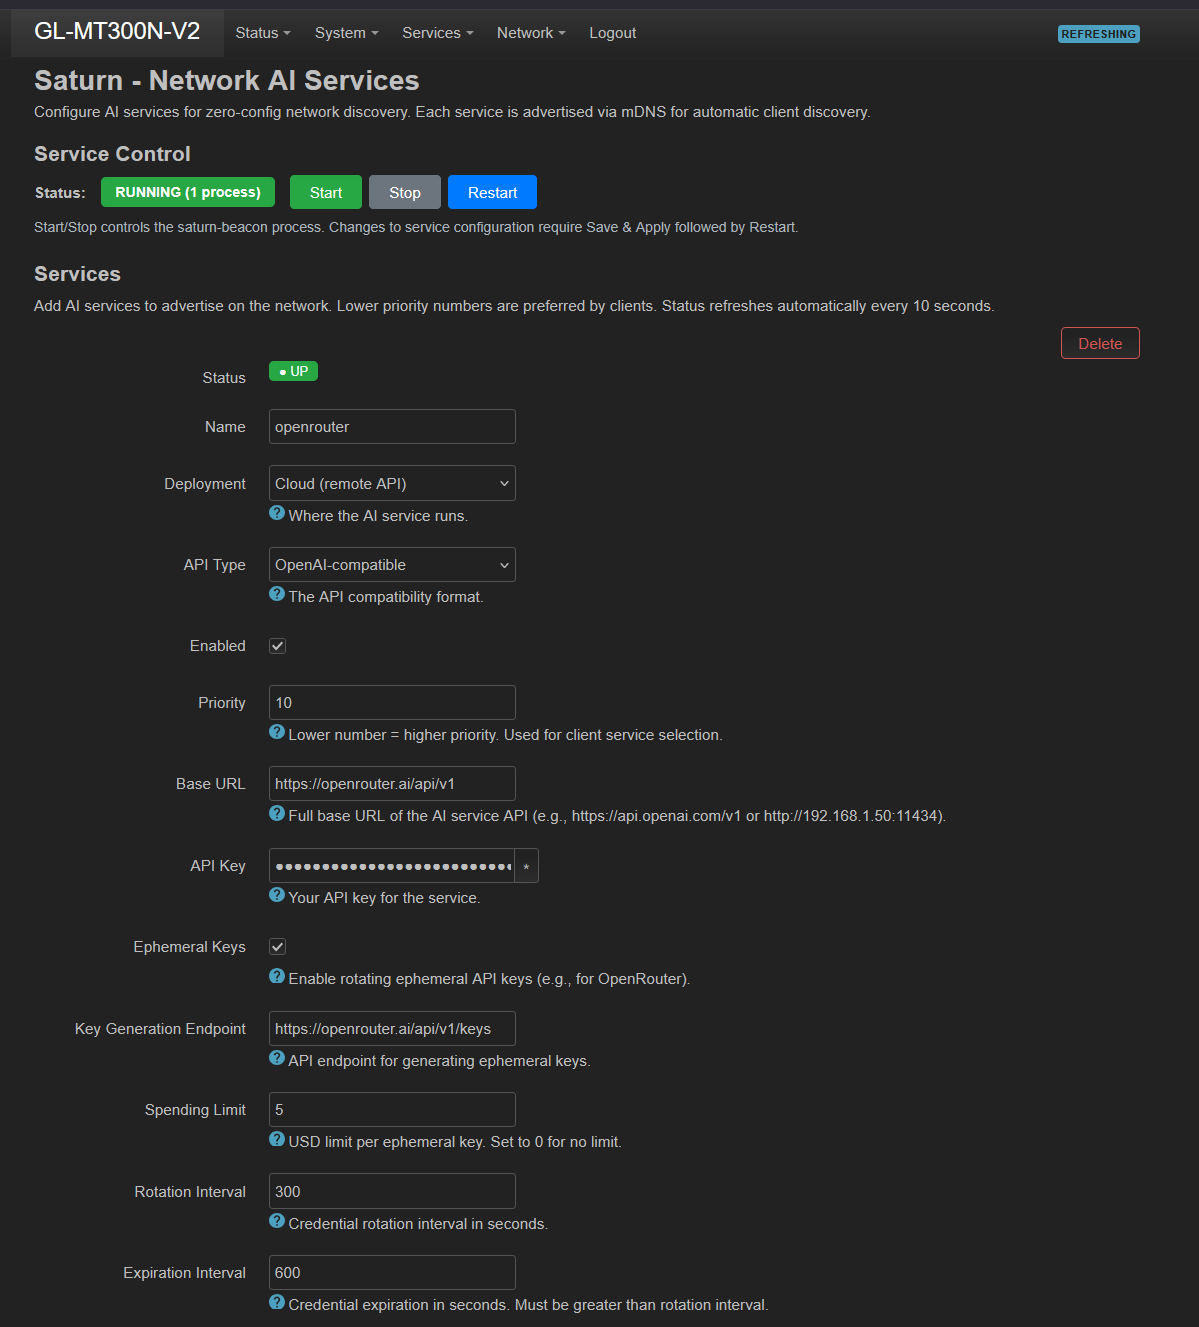
\includegraphics[width=0.85\textwidth]{figures/luci-config.png}
\caption{The Saturn configuration page in LuCI. Each service shows its name, deployment type, upstream endpoint, and a live status badge. Administrators manage Saturn through the same interface they use for DHCP and firewall rules.}
\label{fig:luci-config}
\end{figure}

\section{OpenCode: Saturn in an AI Coding Agent}
\label{sec:opencode-implementation}

While the VLC extension proved Saturn works in a non-AI application, neither it nor the router tests whether Saturn can handle a coding agent asking a model to edit three files, run a shell command, inspect the output, and continue the conversation --- all over a single streaming connection. OpenCode, an open-source terminal-based coding agent built by Anomaly, demands exactly this.
I forked OpenCode because Saturn requires runtime provider registration, a capability its static loader system does not support. The fork adds one capability --- dynamic provider discovery --- without modifying OpenCode's core routing, session management, or rendering. I integrated \texttt{ai-sdk-provider-saturn}\footnote{\url{https://github.com/jperrello/Saturn/tree/main/ai-sdk-provider-saturn}} as a bundled provider.

\subsection{Integration and Dynamic Registration}

I extended OpenCode's existing \texttt{CUSTOM\_LOADERS} provider system rather than forking its core abstractions.
The integration adds a \texttt{saturn} loader entry that creates a discovery instance with a three-second timeout, fetches \texttt{/v1/models} from all discovered services, and registers each model as a dynamic provider.
I touched twelve files across four packages but modified none of OpenCode's core abstractions. Confining changes to the loader layer forced the dynamic registration workaround described below.

Dynamic registration is the central challenge. OpenCode assumes the model set is fixed at startup, but Saturn models appear and disappear at runtime as services come online or fail. I bridged this gap with two callbacks: \texttt{onServiceDiscovered} fetches models from new services and calls \texttt{registerDynamic()}, while \texttt{onServiceRemoved} verifies the removal and calls \texttt{unregisterDynamic()}. Both callbacks emit events on instance-scoped and process-wide buses, updating model selectors in real time. The cost is that any component holding a model reference must tolerate that reference becoming invalid between ticks --- a stale reference fails silently rather than routing to a valid backend. I enforced invalidation through the event bus rather than polling.

Figure~\ref{fig:opencode-saturn} shows the model selector populated with Saturn-discovered models.

\begin{figure}[H]
\centering
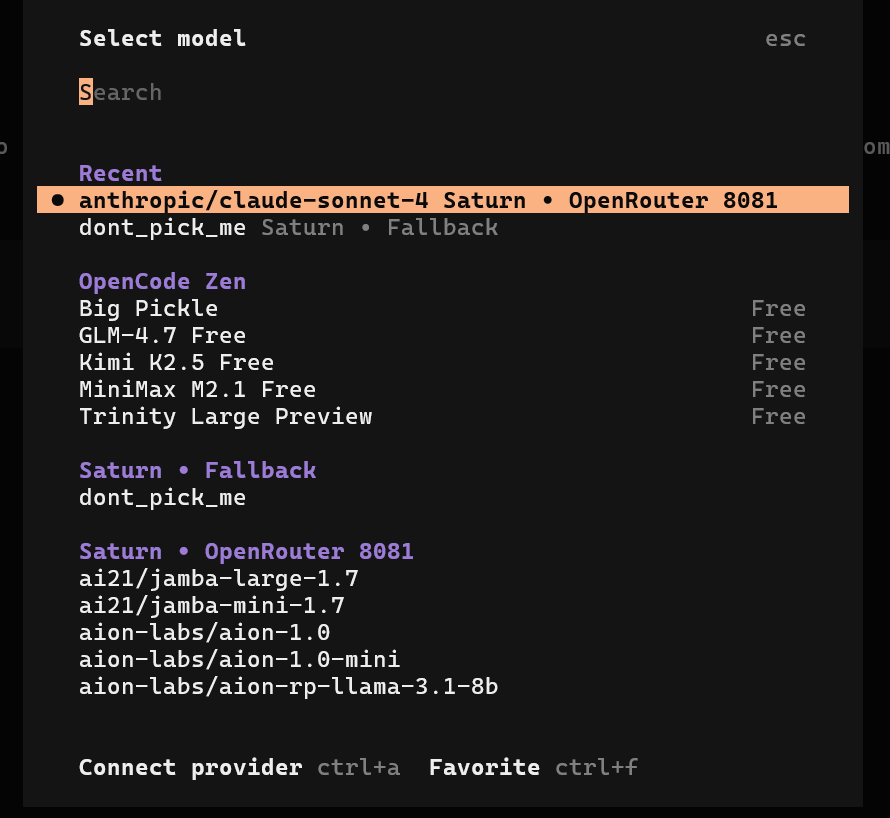
\includegraphics[width=0.85\textwidth]{figures/opencode-saturn.png}
\caption{OpenCode's model selector showing Saturn-discovered models. Each entry is prefixed with its service name (e.g., \texttt{saturn:office/gpt-4o}), populated at runtime through mDNS discovery with no user configuration.}
\label{fig:opencode-saturn}
\end{figure}

Integrating Saturn surfaced six bugs, three critical, and every critical bug traced to the same root cause: the host application assumed providers are configured at startup, not discovered at runtime. The simplest was a \texttt{finishReason} format mismatch: OpenCode expected AI SDK v2's plain string format (\texttt{"stop"}), but Saturn's provider returns v3 objects, fixed by one line of type normalization. Without a \texttt{toolCalling} capability flag, the agent lost the functionality that justified this implementation: OpenCode serialized function calls as plain text instead of invoking the tool-calling protocol, so the agent could chat but could not edit files or run commands; setting \texttt{toolcall: true} in the dynamic registration restored full agentic behavior. The most disruptive bug required the ugliest fix: Bun's default HTTP timeout killed long-running streaming requests, and because Bun provides no per-request timeout override, I monkey-patched \texttt{globalThis.fetch} to disable timeouts during streaming calls.

A concrete session illustrates the integration end-to-end. A developer launches OpenCode-Saturn in a project directory. The Saturn loader discovers two services, fetches their model lists, and populates the selector---the developer sees entries like \texttt{saturn:\allowbreak{}office/\allowbreak{}gpt-4o} without configuring any provider. The developer asks the agent to refactor a function; the agent streams a response while invoking file-edit and shell tools through the standard tool-calling protocol. If the office service goes down mid-session, failover reroutes to the same model on another service or sends an error if none available.

\section{Summary}
\label{sec:impl-summary}

Table~\ref{tab:impl-summary} summarizes the three implementations. Beyond these and the two SDK packages described above, I built two additional integrations: an Open WebUI plugin\footnote{\url{https://github.com/jperrello/Saturn/blob/main/owui_saturn.py}} (one uploaded file replaces per-backend configuration) and an MCP server\footnote{\url{https://github.com/jperrello/Saturn/tree/main/saturn-mcp}} (one JSON config entry exposes Saturn discovery as tools for AI coding assistants). Together, these seven artifacts span three languages and four mDNS libraries: VLC (Lua/Python, \texttt{dns-sd}), the router (Rust, \texttt{mdns-sd}), OpenCode, Open WebUI, and the MCP server (TypeScript/Python, \texttt{multicast-dns} and \texttt{zeroconf}).

\begin{table}[ht]
\centering
\small
\begin{tabular}{p{2.8cm} p{2.0cm} p{2.2cm} p{5.5cm}}
\hline
\textbf{Implementation} & \textbf{Language} & \textbf{mDNS Library} & \textbf{What It Demonstrates} \\
\hline
VLC Extension & Lua / Python & macOS \texttt{dns-sd} CLI & AI in a non-AI-native consumer application via bridge pattern \\
Saturn Router & Rust & \texttt{mdns-sd} crate & AI provisioning at the network infrastructure layer on constrained hardware \\
OpenCode Fork & TypeScript & \texttt{multicast-\allowbreak{}dns} npm & Full agentic AI workflow with tool calling, streaming, and dynamic discovery \\
\hline
\end{tabular}
\caption{Three Saturn implementations demonstrating progressive scope expansion. Each uses a different mDNS library, supporting argument~\argref{A10}: seven consumers across three languages and four mDNS libraries interoperate on \texttt{\_saturn.\_tcp.local.} with no bridging layer.}
\label{tab:impl-summary}
\end{table}

Each implementation answered a question left open by the previous one. Together they span the range from media players to network infrastructure to AI coding agents. Chapter~\ref{ch:evaluation} evaluates what these implementations demonstrate against the claims advanced in Chapter~\ref{ch:introduction}.
